\section{Transmission Control Protocol (TCP)}

TCP brinda servicios a las aplicaciones, pero es orientado a conexión. Esto agrega:

\begin{itemize}[label=\textcolor{acento}{$\bullet$}]
    \item Confiabilidad
    \item Ordenado
    \item Control de flujo
    \item Control de congestión
    \item Byte stream
\end{itemize}

Las aplicaciones envían streams de bytes. TCP hace la \textbf{packetization:} convierte el stream en un conjunto de mensajes que IP puede transportar. 

Después decide el tamaño de cada \textbf{chunk} para que no tenga que ser fragmentado. Estos chunks se llaman \textbf{segmentos}. Los segmentos contienen información sobre la posición en el stream, además del proceso origen del nodo emisor y el proceso destino en el nodo destino.

\subsection{Segmento de TCP}

El header del segmento tiene esta forma:

\begin{figure}[htbp]
    \centering
    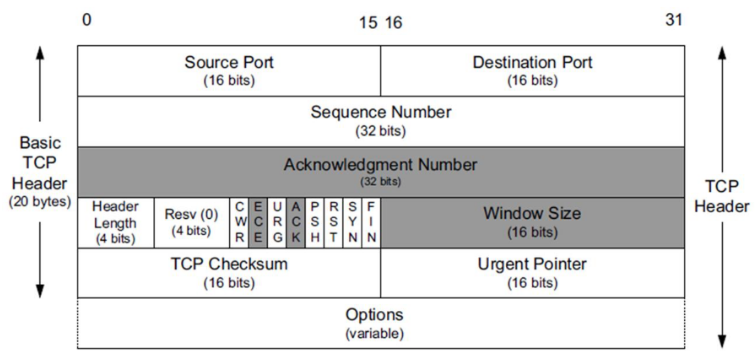
\includegraphics[width=0.7\textwidth]{capitulos/tcp/imagenes/segmento-tcp.png}
    \caption{Segmento TCP}
    \label{fig:segmento-tcp}
\end{figure}

Y sus campos son los siguientes:

\begin{table}[H]
    \centering
    \caption{Campos de la cabecera TCP}
    \label{tab:campos-tcp}
    \renewcommand{\arraystretch}{1.2}
    \begin{tabular}{|p{0.23\textwidth}|p{0.12\textwidth}|p{0.55\textwidth}|}
        \hline
        \textbf{Campo} & \textbf{Tamaño} & \textbf{Descripción} \\ \hline
        Source Port & 16 bits & Indica el número de puerto de la aplicación en el nodo que envía el segmento. \\ \hline
        Destination Port & 16 bits & Indica el número de puerto de la aplicación que debe recibir el segmento. \\ \hline
        Sequence Number & 32 bits & Indica el número asignado al primer byte de datos contenidos en el segmento. \\ \hline
        Acknowledgment Number & 32 bits & Indica el siguiente número de byte que el emisor del segmento espera recibir del otro extremo. \\ \hline
        Header Length & 4 bits & Indica el número de palabras de 4 bytes de la cabecera TCP (entre 20 y 60 bytes). \\ \hline
        Control Bits (Flags) & Variable & También conocidos como \textit{flags}; indican la finalidad del segmento. \\ \hline
        Window Size & 16 bits & Indica la cantidad de bytes, a partir del número de reconocimiento en el segmento, que el emisor puede recibir. \\ \hline
        Checksum & 16 bits & Su cálculo es obligatorio y se realiza sobre todo el segmento más una pseudocabecera. \\ \hline
        Urgent Pointer & 16 bits & Válido si el flag \texttt{U} está seteado. Define el valor a sumar al número de secuencia que indica dónde finalizan los datos urgentes. \\ \hline
        Options & Hasta 40 bytes & Información opcional. \\ \hline
    \end{tabular}
\end{table}

\subsection{Three-Way Handshake}

Se intercambian \textbf{tres segmentos}, donde se indican puertos origen y destino.

\begin{figure}[htbp]
    \centering
    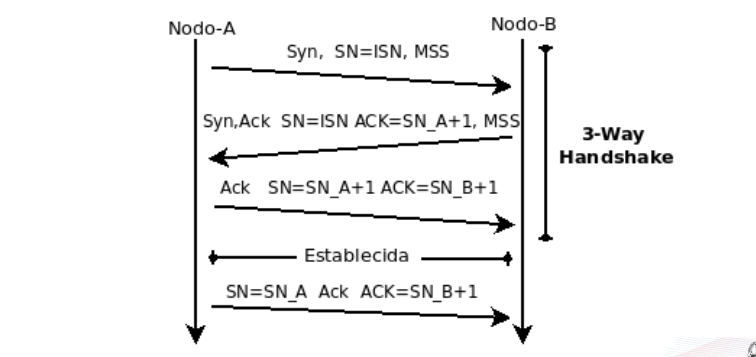
\includegraphics[width=0.7\textwidth]{capitulos/tcp/imagenes/3-way-handshake.png}
    \caption{Three-Way Handshake}
    \label{fig:handshake-tcp}
\end{figure}

\subsubsection{Reset de Conexiones}

Se indica con el \textbf{Flag R} en un segmento, que provoca el cierre inmediato de la conexión. Este reset se puede hacer el cualquier momento, y TCP también lo puede hacer ante determinados eventos. 

El reset es enviado cuando se recibe un segmento que \textbf{no corresponde} a la conexión referenciada. También se envía si se recibe un intento de conexión a un \textbf{puerto cerrado}, a la cual se debe responder con \texttt{Flags R(reset), A (Ack)}.

\subsubsection{Fin de Conexión}

Se intercambian 3 o 4 segmentos para finalizar la conexión, y caulquier extremo puede iniciar el cierre. 

\begin{figure}[htbp]
    \centering
    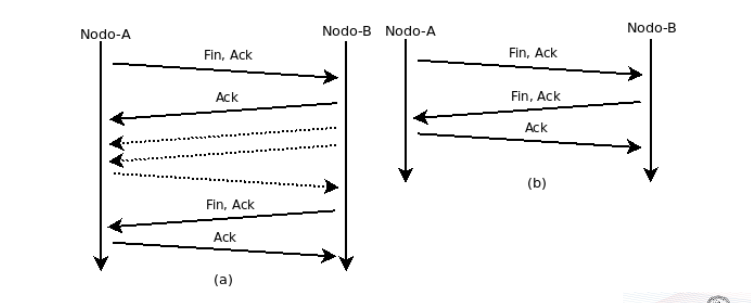
\includegraphics[width=0.7\textwidth]{capitulos/tcp/imagenes/fyn.png}
    \caption{Finalización en TCP}
    \label{fig:fyn-tcp}
\end{figure}

\subsubsection{Estados de TCP}

Durante la conexión, los nodos transitan distintos estados.

\begin{figure}[H]
    \centering
    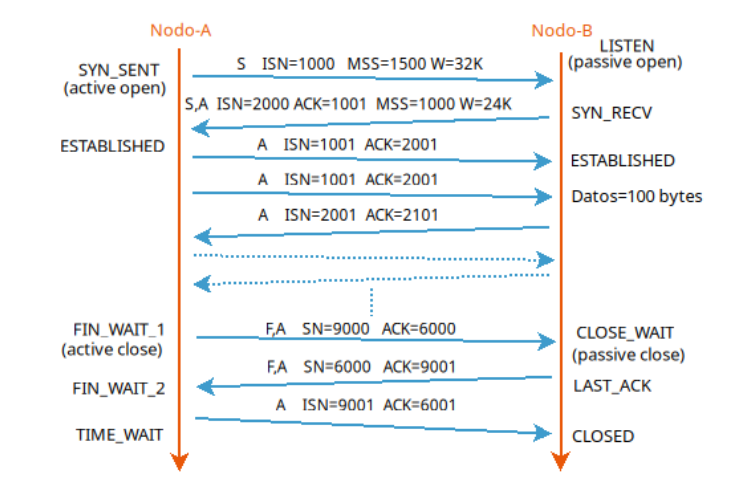
\includegraphics[width=0.7\textwidth]{capitulos/tcp/imagenes/estados-tcp.png}
    \caption{Estados en TCP}
    \label{fig:estados-tcp}
\end{figure}

\begin{nota}{\textbf{\emph{Recordar...}}\newline}
    Las conexiones TCP empiezan con un \textbf{Three-Way Handshake}, con los flags
    
    \begin{enumerate}[label=\textcolor{acento}{\textbf{\arabic*.}}]
        \item SYN
        \item SYN, ACK
        \item ACK
    \end{enumerate}

    El \textbf{Flag de Reset (R)} provoca un cierre instantáneo de una conexión, que se puede volver a abrir. 
    
    Para el \textbf{cierre correcto} de una conexión, también hay un intercambio de 3/4 mensajes.
\end{nota}

\subsection{Intercambio de Datos}

\begin{definicion}{Maximum Segment Size (MSS)}
    Es la máxima longitud de segmento que se puede recibir sin contar la cabecera. Es una opción mandatoria, no es un campo en el header. Se envía en el three-way handshake. 

    Es diferente para \textbf{cada sentido de la conexión}.
\end{definicion}

TCP tiene una \textbf{pseudocabecera} que se construye localmente para el cálculo del checksum. Sirve para verificar la integridad del segmento.

Los \textbf{sequence numbers} son un número de 32 bits cuyo valor de \textbf{ISN} (initial sequence number) se determina localmente en cada extremo. Cada byte enviado sobre una conexión TCP tiene un número de secuencia, y se incrementa según los bytes transmitidos y reconocidos. Indica la ubicación de cada byte en el stream.

\begin{figure}[htbp]
    \centering
    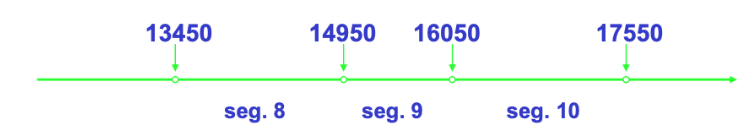
\includegraphics[width=0.7\textwidth]{capitulos/tcp/imagenes/secuencia.png}
    \caption{Secuencias en TCP}
    \label{fig:secuencia-tcp}
\end{figure}

Es un canal \textbf{Full-Duplex} (bidireccional), donde un extremo puede enviar datos hasta que alcance el tamaño de la ventana de recepción sin esperar un ACK. 

El número de ACK indica el siguiente byte que se espera recibir. Si el segmento llega con errores, es retransmitido. 

\begin{nota}{\textbf{\emph{recordar}}\newline}
    Puedo enviar datos hasta llegar a la ventana de transmisión sin tener que esperar un ACK. Si el segmento no tiene errores, me tienen que enviar un ACK. Sino, tengo que retransmitir.
\end{nota}

\subsection{Control de Flujo}

Cada extremo anuncia el tamaño de su \textbf{ventana de recepción} al inicio de la sesión, y pueden ser \textbf{distintos}.

Se utiliza para que un extremo no envíe datos más rápido de lo que el otro extremo los pueda procesar. Si los datos no son leídos por la aplicación, el extremo debe anunciar su ventana de recepción con un menor tamaño.  

\begin{figure}[H]
    \centering
    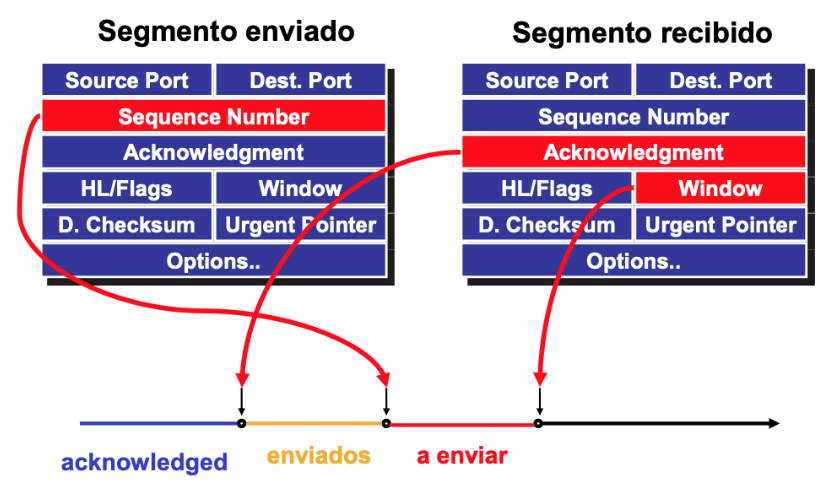
\includegraphics[width=0.7\textwidth]{capitulos/tcp/imagenes/ventana-deslizante.png}
    \caption{Ventana deslizante en TCP}
    \label{fig:ventana-deslizante}
\end{figure}

\begin{definicion}{RTO y RTT}
    \textbf{Round Trip Time:} es el tiempo entre que se envía un segmento y ACK de reconocimiento. El RTT varía continuamente.

    \textbf{Retransmission TimeOut:} el tiempo que debe pasar para retransmitir un paquete. 
\end{definicion}

El \textbf{Maximum Segment Size} se comunica en el campo de \textbf{opciones}, al igual que el escalado de la ventana (\textbf{TCP Windows Scale}). El scale se envía al inicio de sesión, y se va modificando. 

\subsubsection{Timers}

El \textbf{Persist Timer} se utiliza cuando la ventana de recepción se reduce a cero. Una vez que se reduce la ventana, el emisor va enviando paquetes de \textbf{1 Byte} cada un intervalo de tiempo que va incrementando (\textbf{Back-Off}). Esto se hace hasta no recibir un \texttt{ACK} con \texttt{wind = 0}.

El \textbf{Keepalive Timer} sirve para mantener una conexión abierta cuando no hay intercambio de datos. Se utiliza para interrogar al otro extremo por su estado, y funciona de forma muy similar al \emph{persist timer}.